\chapter{Binarisierung}
\section{Binarisierung der Bilder}
Das Binarisieren der importierten Bilder stellt die erste Hürde im Binarisierungsprozess des \textit{NNs} auf. Wir arbeiten in unserem \textit{BNN} mit \textit{Grey-Scaled}-Bildern, d.h. wir verarbeiten nur einen $\alpha$\textit{-Kanal} anstatt drei \textit{RGB-Kanälen}. Dieser $\alpha$\textit{-Kanal} bewegt sich jedoch in einem Wertebereich von $\{0-255\}$ bzw. $(0,1)$ mit einer Granularität von $\frac{1}{255}$.\\

Unsere Aufgabe bei der Binarisierung ist es also mit möglichst wenig Informationsverlust eine Funktion $\mathbb{Q}_{0-1} \rightarrow \{0,1\}$ zu entwickeln, die unsere importierten Bilder binarisiert.

\subsection{Threshold}

Im Folgenden betrachten wir den Wertebereich der Pixel als zwischen $\{0-255\}$ liegend.\\Der erste Ansatz für eine Binarisierungsfunktion betrachten wir Thresholds. Diese Funktion flippt für ein fest gewähltes $n \in \{0..255\}$ alle Bits, die den Schwellenwert $n$ überschreiten, auf $1$ und alle anderen auf $0$.\\

Der Vorteil dieser Methode ist, dass man eine sehr kostengünstige Binarisierung erhält (150ms pro 100 Bilder). Man kann durch das fest gewählte $n$ die \textit{Inbuild}-Tensor-Funktionen verwenden und muss nicht manuell über die einzelnen Pixel iterieren. Dies ist vorallem wichtig, da man mit $60.000$ Bildern je $28 \times 28$ Pixeln sehr viele Binarisierungsschritte je Epoche erhält.\\

Der große Nachteil an der Threshold-Methode ist, dass man kompromisse machen muss. Es gibt nicht einen guten Threshhold, da für jeden gewählten Threshold bei einer Teilmenge der Bilder zuviel, bzw. zu wenig gefiltert wird. (Siehe Abbildung 5.1 bzw. 5.2)
\begin{figure}[h]
\centering
\begin{minipage}{.5\textwidth}
  \centering
  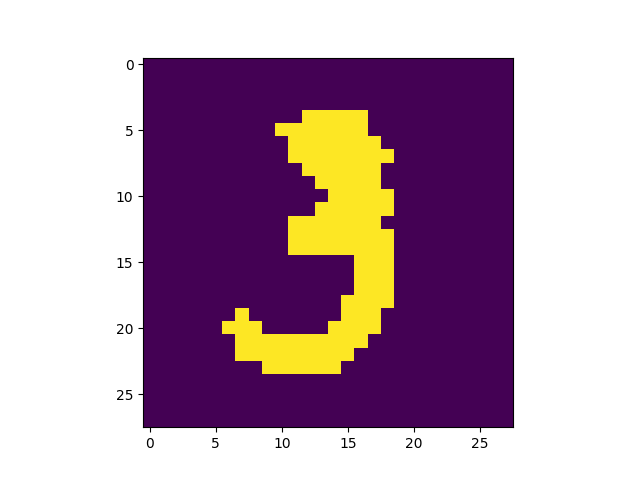
\includegraphics[width=.4\linewidth]{./bilder/comparison/threshold/100_3}
  \captionof{figure}{3, Threshold 100}
  \label{fig:bin3}
\end{minipage}%
\begin{minipage}{.5\textwidth}
  \centering
  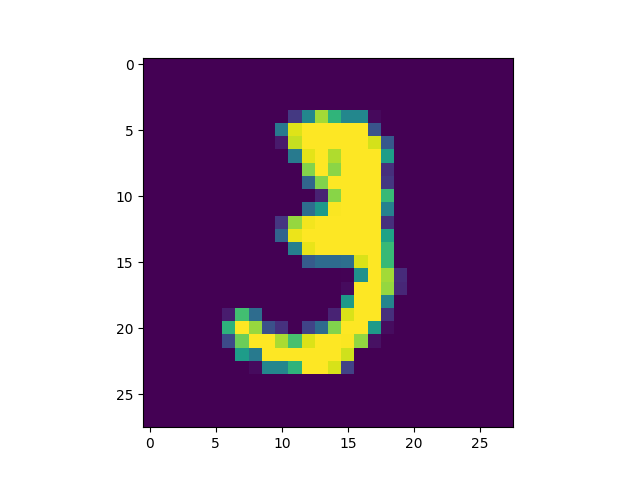
\includegraphics[width=.4\linewidth]{./bilder/comparison/default_3}
  \captionof{figure}{3, not binarized}
  \label{fig:dflt}
\end{minipage}
\begin{minipage}{.5\textwidth}
  \centering
  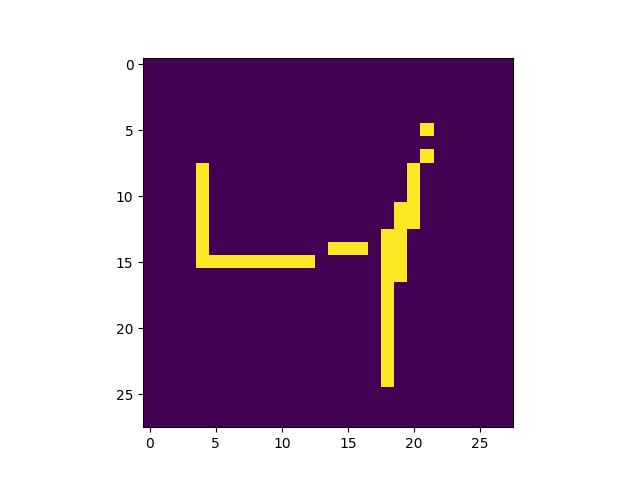
\includegraphics[width=.4\linewidth]{./bilder/comparison/threshold/200}
  \captionof{figure}{4, Threshold 200}
  \label{fig:bin4}
\end{minipage}%
\begin{minipage}{.5\textwidth}
  \centering
  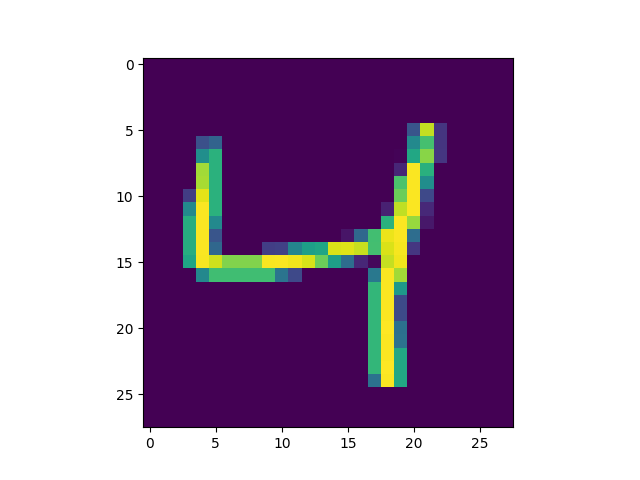
\includegraphics[width=.4\linewidth]{./bilder/comparison/default}
  \captionof{figure}{4, not binarized}
  \label{fig:dflt}
\end{minipage}

\end{figure}
In diesem Vergleich sieht man sehr gut, dass ein Threshold, der für ein Bild zu tief gesetzt ist, d.h. es werden zu wenig Pixel gefiltert nicht erhöht werden kann, da er sonst für ein anderes Bild zu hoch gesetzt ist(es werden zu viele Pixel gefiltert).\\

\subsection{Probability}

Eine Lösung für dieses Problem bietet die \textit{Probability-Transformation}. Bei dieser Methode betrachten wir den Wert eines einzelnen Pixels als die Wahrscheinlichkeit, dass dieser Pixel in der Binarisierung mit $1$ belegt wird. So werden Pixel mit den Wert $255$ immer mit $1$ belegt und Pixel mit dem Wert $130$ ungefähr $50\%$ der Zeit.\\

Nachteil dieser Methode ist die Effizienz. Da wir nun nicht mehr mit einem statischen Threshold arbeiten, müssen wir manuell über die Pixel iterieren. Dabei verschlechtern wir uns im Zeitlichen um einen Faktor $20$. Selbst nach großen Optimierungen in Form von Tensor-Umwandlung in Numpy-Arrays und Numba-Integration dauert die \textit{Probability-Transformation} doppelt solange wie die \textit{Threshold-Transformation}. Zu dem konvergiert die Probability Methode erst nach Rund $600$ Epochen wohingegen die Threshold-Methode nur rund $100$ Epochen benötigt. Somit ist das Trainieren mit der \textit{Probability-Transformation} deutlich teurer.\\

Der große Vorteil dieser Methode ist jedoch die Informationserhaltung. Wir arbeiten bei der \textit{Probability-Transformation} mit sogenannten \textit{Repetitions}. Diese durchlaufen die gleiche Generation mit dem gleichen \textit{Trainingset}, welche jedoch neu binarisiert wurden. Das heißt, dass man bei 50 Repetitions jede Generation 50 mal, mit 50 unabhängig binarisierten \textit{Trainginsets} durchläuft.\\Dadurch erhalten wir ein Mittel für jedes Bild, welches gegen die Originalversion konvergiert. (Siehe Abbildung 5.5 bzw 5.6)

\begin{figure}[h]
\centering
\begin{minipage}{.5\textwidth}
  \centering
  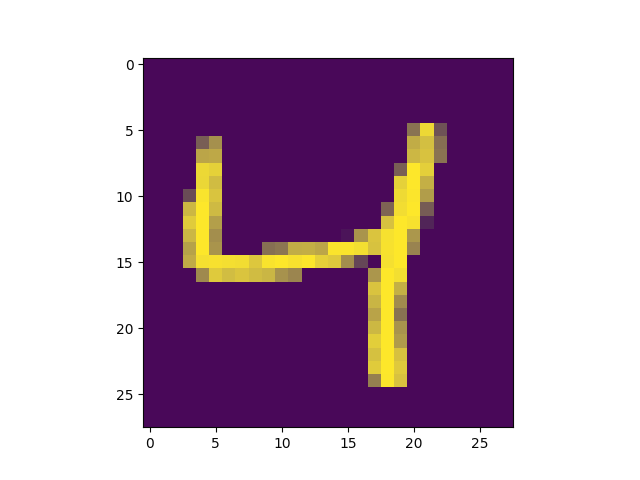
\includegraphics[width=.4\linewidth]{./bilder/comparison/overlapped}
  \captionof{figure}{4, overlapped 50 prob-trans}
  \label{fig:bin3}
\end{minipage}%
\begin{minipage}{.5\textwidth}
  \centering
  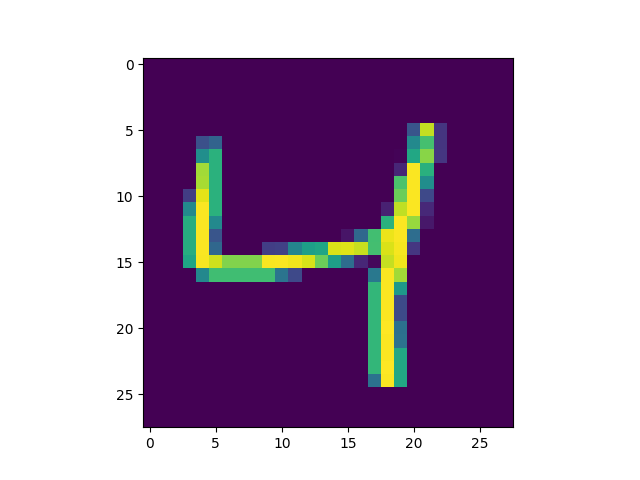
\includegraphics[width=.4\linewidth]{./bilder/comparison/default}
  \captionof{figure}{4, not binarized}
  \label{fig:dflt}
\end{minipage}
\end{figure}

\subsection{Evaluation}

Um die verschiedenen Methoden zu Vergleichen, haben wir beide Transformationen und eine Referenzinstanz für $600$ Epochen, bzw. 20 Epochen und 30 Repetitions, trainieren lassen.\\

	
	\begin{tabular}{|c|c|c|c|}\hline
		\centering
		Run & Non-Binarized    & threshold        & prob              \\\hline
		1   	& 91.99\%          & 89.24\%          & 92.52\%           \\\hline
		2   & 91.99\%          & 89.24\%          & 91.82\%           \\\hline
		3   & 91.99\%          & 89.24\%          & 92.56\%           \\\hline
		4   & 91.99\%          & 89.24\%          & 91.02\%           \\\hline
		avg & \textbf{91.99\%} & \textbf{89.24\%} & \textbf{91.98\%}  \\\hline
	\end{tabular}
	\captionof{figure}{Vergleich}
	\label{fig:grph}

Es ist gut zu erkennen, dass bei der Binarisierung mit der \textit{Threshold}-Methode über $2\%$ Genauigkeit verloren wird. Zudem sind unsere Referenzinstanz und die \textit{Threshold}-Methode bereits konvergiert, heißt sie erzielen keine Verbesserung mehr.\\
 Die \textit{Probability-Transformation} schwankt jedoch noch in der Genauigkeit. Dies liegt überwiegend an der Varianz in der Binarisierung bedingt durch die Wahrscheinlichkeit. Trotz dieser Varianz ist zu erkennen, dass das Mittel der \textit{Probability-Transformation} gegen unsere Referenzinstanz konvergiert. Somit haben wir eine Transformation, bei der wir durch zeitliche Einbuße keine Genauigkeitsverluste verzeichnen müssen.\\
 
Nun sind die zeitlichen Einbuße, durch den Faktor $12$ beschrieben, so groß, dass es sich nicht lohnt bei dem Testen von Parametern oder Ausprobieren von Konzepten mit der \textit{Probability-Transformation} zu arbeiten. In diesen Fällen ist es effizienter die $2\%$ Genauigkeitsverlust in Kauf zu nehmen und deutlich schnelle arbeiten zu können. Es hilft uns im Finalen Netz aber durchaus unsere Hürde von $90\%$ zu überschreiten.


